\section*{Програмний етап}
\addcontentsline{toc}{section}{Програмний етап}

Для статистичного аналізу було обрано відкриті дані із загальнодоступного освітнього сайту 
\url{https://osvita.ua/news/data/}, де з-поміж інших наборів даних у переліку доступні 
<<Деперсоніфіковані дані учасників ЗНО 2019 року з кожного навчального предмета>>.

\subsection*{Ініціалізація даних}
\addcontentsline{toc}{subsection}{Ініціалізація даних}

Зі сторінки сайту можна завантажити архів даних \texttt{opendatazno2019.zip}. У роз\-архівованій папці 
наявні два файли з різними іменами: \texttt{opendatazno2019.xlsx} та \texttt{opendatazno2019\_info.xls}. 
У першому містяться власне дані, а у другому -- перелік атрибутів таблиці даних.  

Файл \texttt{opendatazno2019.xlsx} має великий обсяг -- понад $230\ \text{MB}$, тому жоден онлайн редактор не 
буде в змозі його відкрити. Рівно як і програмне забезпечення \texttt{Microsoft Excel}, \texttt{Google Sheets} 
чи \texttt{LibreOffice Calc}. Тож для подальшого опрацювання вхідних даних буде використано засоби мови \texttt{Python}. 

Для читання файлів розширення \texttt{.xlsx} можна використати бібліотеку \texttt{xlrd} версії \texttt{1.2.0} 
й надалі працювати безпосередно із рядками таблиці, пробігаючи кожну комірку так, як це показано у рядку $13$ 
Лістингу  \ref{code: xlrd}:

% in case you want to paste code from a file:
% \lstinputlisting[firstnumber=1, firstline=1, lastline=14, label = code: xlrd, caption = Використання бібліотеки xlrd]{conversion_stage.py}

\begin{lstlisting}[firstnumber=1, label = code: xlrd, caption = Використання бібліотеки xlrd]
import xlrd

# open the workbook
workbook = xlrd.open_workbook("opendatazno2019.xlsx")
    
# open the worksheet
worksheet = workbook.sheet_by_index(0)
    
# iterate the rows and columns
for i in range(0, 5):
    for j in range(0, 3):
        # print the cell values with a tab space
        print(worksheet.cell_value(i, j), end="\t")
    print("")
\end{lstlisting}

\vspace{0.4cm}
Проте у такому разі обробка файлу триватиме близько $5$-ти хвилин, тож такий спосіб опрацювання великого 
обсягу даних є неефективним. Натомість, користуючись тією ж бібліотекою \texttt{xlrd} у додачу до засобів 
бібліотек \texttt{pandas} та \texttt{csv}, можна зчитати й порядково перевторити файл розширення \texttt{.xlsx} 
у файл \texttt{.csv}, як це наведено на Лістингу \ref{code: .xlsl to .csv}. Це значно зменшить тривалість 
виконання обробки даних. Більше про різні способи зчитування й обробки файлів розширення \texttt{.xlsx} можна 
довідатися за \href{https://linuxhint.com/read-excel-file-python/}{цим посиланням}.

\newpage
\begin{lstlisting}[firstnumber=16, label = code: .xlsl to .csv, caption = Конвертація у \texttt{.csv} файл]
import pandas as pd
import xlrd 
import csv
    
# open workbook by sheet index, optional - sheet_by_index()
sheet = xlrd.open_workbook("opendatazno2019.xlsx").sheet_by_index(0)
    
column = csv.writer(open("opendatazno2019.csv", "w", newline=""))
    
# row by row rewrite the data into csv file
for row in range(sheet.nrows):
    column.writerow(sheet.row_values(row))
    
# convert file into a dataframe object
df = pd.DataFrame(pd.read_csv("opendatazno2019.csv", dtype="unicode"))
\end{lstlisting}

\vspace{0.4cm}
Як це зображено на Рис. \ref{figure: initial data}, початкові дані мають рядки невідповідного формату, 
тобто ці дані є <<брудними>>. На Лістингу \ref{code: cleaning data} коротко вказані команди, за допомогою 
яких можна прибрати нульові значення чи комірки з невідповідним форматом. Як результат -- матимемо готові 
<<чисті>> дані для подальшої обробки. 

\begin{figure}[H]
    \center{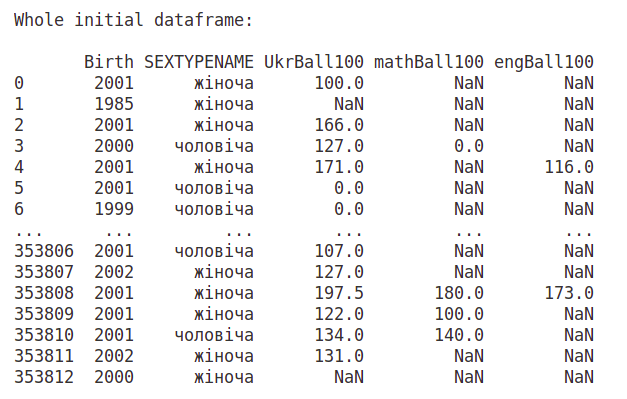
\includegraphics[width=1\linewidth]{Initial data 14.png}}
    \caption{Початкові дані}
    \label{figure: initial data}
\end{figure}

\begin{lstlisting}[firstnumber=36, label = code: cleaning data, caption = Чистка даних]
df = pd.DataFrame(pd.read_csv("opendatazno2019.csv", dtype="unicode"))

# remove all rows with NULL values:
cleaned_df = df.dropna(subset=["UkrBall100"])

# reset indexes after removing rows from the dataframe
cleaned_df = cleaned_df.reset_index(drop=True)

# convert strings to floats in order to use .mean() later
cleaned_df["UkrBall100"] = cleaned_df["UkrBall100"].astype("float") 

# select rows without "0.0" values:
cleaned_df = cleaned_df.loc[cleaned_df["UkrBall100"] != 0.0]
cleaned_df.reset_index(drop=True, inplace=True)
\end{lstlisting}

\subsection*{Реалізація рандомізованого формування елементів вибірок}
\addcontentsline{toc}{subsection}{Реалізація рандомізованого формування елементів вибірок}

Важливим етапом статистичного аналізу є реалізація випадкового, рандомізованого формування вибірок із усього 
наявного масиву даних. Програмно таку реалізацію наведено на Лістингу нижче.

\begin{lstlisting}[firstnumber=51, label = code: randomization, caption = Рандомізоване формування вибірок]
import random

sample_size = 500

# create a list of all the possible indexes
index = [i for i in range(0,cleaned_df.last_valid_index()+1)]

# create an empty dictionary
random_elements = {}

# add one empty column to the dictionary
elements = []
random_elements.update({"UkrBall100": elements})

for i in range(sample_size):
    random_index = random.choice(index)
    elements.append(cleaned_df.loc[random_index, "UkrBall100"])
    index.remove(random_index)

# convert dictionary to a dataframe
random_selected_df = pd.DataFrame(random_elements)
\end{lstlisting}

\vspace{0.4cm}
Із усім використаним в ході роботи програмним кодом \texttt{Python} можна ознайомитися на  
\href{https://github.com/Arroneq/SA-PYTHON.git}{\texttt{github репозиторії}}.